%! Author = Filippo Vissani
%! Date = 08/02/24
% !TeX root = ../thesis-main.tex

%----------------------------------------------------------------------------------------
\chapter{Design}
\label{chap:design}
%----------------------------------------------------------------------------------------

This chapter delves into the design of a reactive extension for the Collektive framework. Collektive enables the execution of aggregate computations across distributed devices. This chapter introduces two novel models that incorporate reactive principles into Collektive's design.

The chapter begins by providing an overview of the current Collektive architecture. It then outlines the proposed reactive architecture, highlighting the introduced components and their functionalities.

Following the architectural overview, the chapter dives into the detailed design of two reactive models proposed.

\section{Architecture}

As mentioned in \Cref{subsection:collektive-architecture}, Collektive consists of three main modules: \texttt{dsl}, \texttt{compiler-plugin} and \texttt{alchemist-incarnation-collektive}. \texttt{alchemist-incarnation-collektive} is responsible for enabling the integration of Collektive simulations into Alchemist. The \texttt{compiler-plugin} takes care of visiting the abstract syntax tree of the aggregate expression and modifying the function call stack to correctly align the devices that execute the aggregate program. The \texttt{dsl} module defines the following components:
\begin{itemize}
    \item \texttt{aggregate}: deals with defining the context related to a device, the semantics of aggregate constructs, and the data structures necessary for path definition and device alignment;
    \item \texttt{field}: Contains the definition of computational field and the related functionalities for manipulating the latter;
    \item \texttt{state}: defines the association between the paths and the results of their evaluations;
    \item \texttt{path}: Defines the data structures necessary to represent the abstract syntax tree relating to the aggregate expression;
    \item \texttt{networking}: defines the data structures necessary for distributed device communication.
\end{itemize}

Given the solutions proposed in \Cref{subsection:integration-solutions-identified}, in both cases, it is necessary to review some of the entities present in Collektive so that it is possible to detect and react to their changes. Regardless of the detailed solution chosen, given that the Collektive design allows it, it is possible to introduce the necessary functionalities as an extension of the current ones. The proposed architecture is shown in \Cref{fig:collektive-prm-architecture}, the components in gray are part of the current Collektive architecture, and those in orange introduce the entities that enable reactive aggregate programming. The component \texttt{reactive} extends \texttt{aggregate} to introduce a reactive version of the entities described above and \texttt{network} to allow reactive distributed communication between devices. The component \texttt{flow.extensions} is used to simplify some operations for combining and mapping flows. According to this design choice, the other modules in the project (\texttt{compiler-plugin} and \texttt{alchemist-incarnation-collektive}) are not altered; consequently, the reactive model introduced continues to make use of the compiler plugin for the definition of the paths.

\begin{figure}
    \centering
    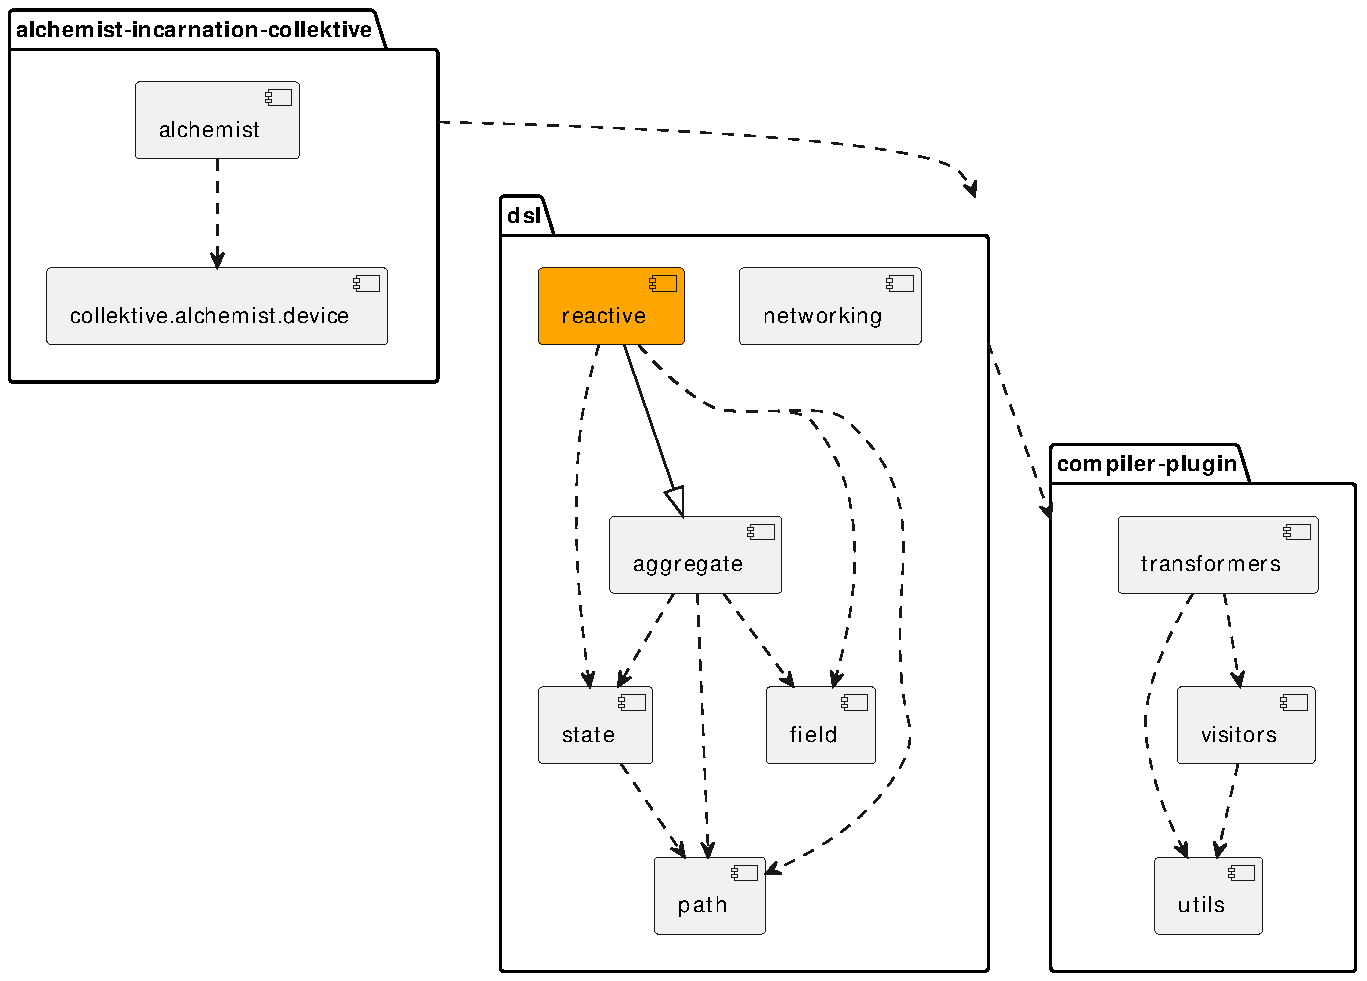
\includegraphics[width=\linewidth]{figures/collektive-prm-architecture.pdf}
    \caption{Architecture of the reactive model proposed. The gray-colored components are part of the original Collektive architecture, while the orange-colored components are used to introduce the reactive paradigm.}
    \label{fig:collektive-prm-architecture}
\end{figure}

\section{Detailed Design}

\subsection{Purely Reactive Model}
\label{subsection:purely-reactive-model}

The detailed design of the purely reactive model is shown in \Cref{fig:collektive-prm-design}.

Within the \texttt{RCollektive} class, the methods for executing aggregate programs have been augmented to accommodate reactive functionalities. The method \texttt{execute} now takes a \texttt{MutableStateFlow<List<InboundMessage<ID>>>} parameter, enabling the system to react to incoming messages from neighboring devices. Similarly, the \texttt{execute} method now also accepts a \texttt{ReactiveNetwork<ID>} parameter, facilitating reactive communication among devices within the network. These additions signify a departure from the static nature of traditional aggregate computations, allowing for dynamic adjustments based on real-time changes in the environment.

In the purely reactive model, the concept of expression result (\texttt{RAggregateResult}) is revisited to imbue reactivity. This ensures that the aggregate expression's result is not static but rather dynamic, adapting to alterations in the underlying data or environmental conditions. Moreover, the \texttt{Aggregate} interface undergoes modifications to accommodate reactive versions of aggregate constructs. Parameters within these constructs are bound to \texttt{StateFlow}, enabling reevaluation whenever their inputs experience changes. This reactive paradigm empowers the system to respond dynamically to fluctuations in the environment.

The \texttt{RAggregateContext} class extends the \texttt{Aggregate} interface, providing concrete implementations of reactive aggregate constructs. Additionally, it hosts reactive data structures essential for managing outbound messages and states. Leveraging \texttt{StateFlow} extensions (\texttt{StateFlowExtensions}), this class simplifies the mapping and combining of hot flows, enhancing the efficiency and scalability of the system. By encapsulating reactive functionalities within the \texttt{RAggregateContext}, the system maintains modularity and extensibility, facilitating future enhancements and optimizations.

\subsubsection{Behavioral Characteristics}

The purely reactive model exhibits distinct behavioral characteristics that distinguish it from traditional static computation approaches:

\begin{itemize}
    \item \textbf{Reactive Computations}: Computation occurs reactively in response to environmental changes, minimizing resource wastage and ensuring optimal responsiveness.
    \item \textbf{Efficient Message Exchange}: Devices only broadcast messages when necessary, reducing unnecessary communication.
    \item \textbf{Selective Reevaluation}: Sub-expressions are reevaluated only when their dependencies change, optimizing computation efficiency and reducing redundant processing.
\end{itemize}

By embodying these characteristics, the purely reactive model enhances the agility, scalability, and robustness of the Collektive framework, empowering it to effectively handle dynamic and unpredictable environments.

\begin{figure}
    \centering
    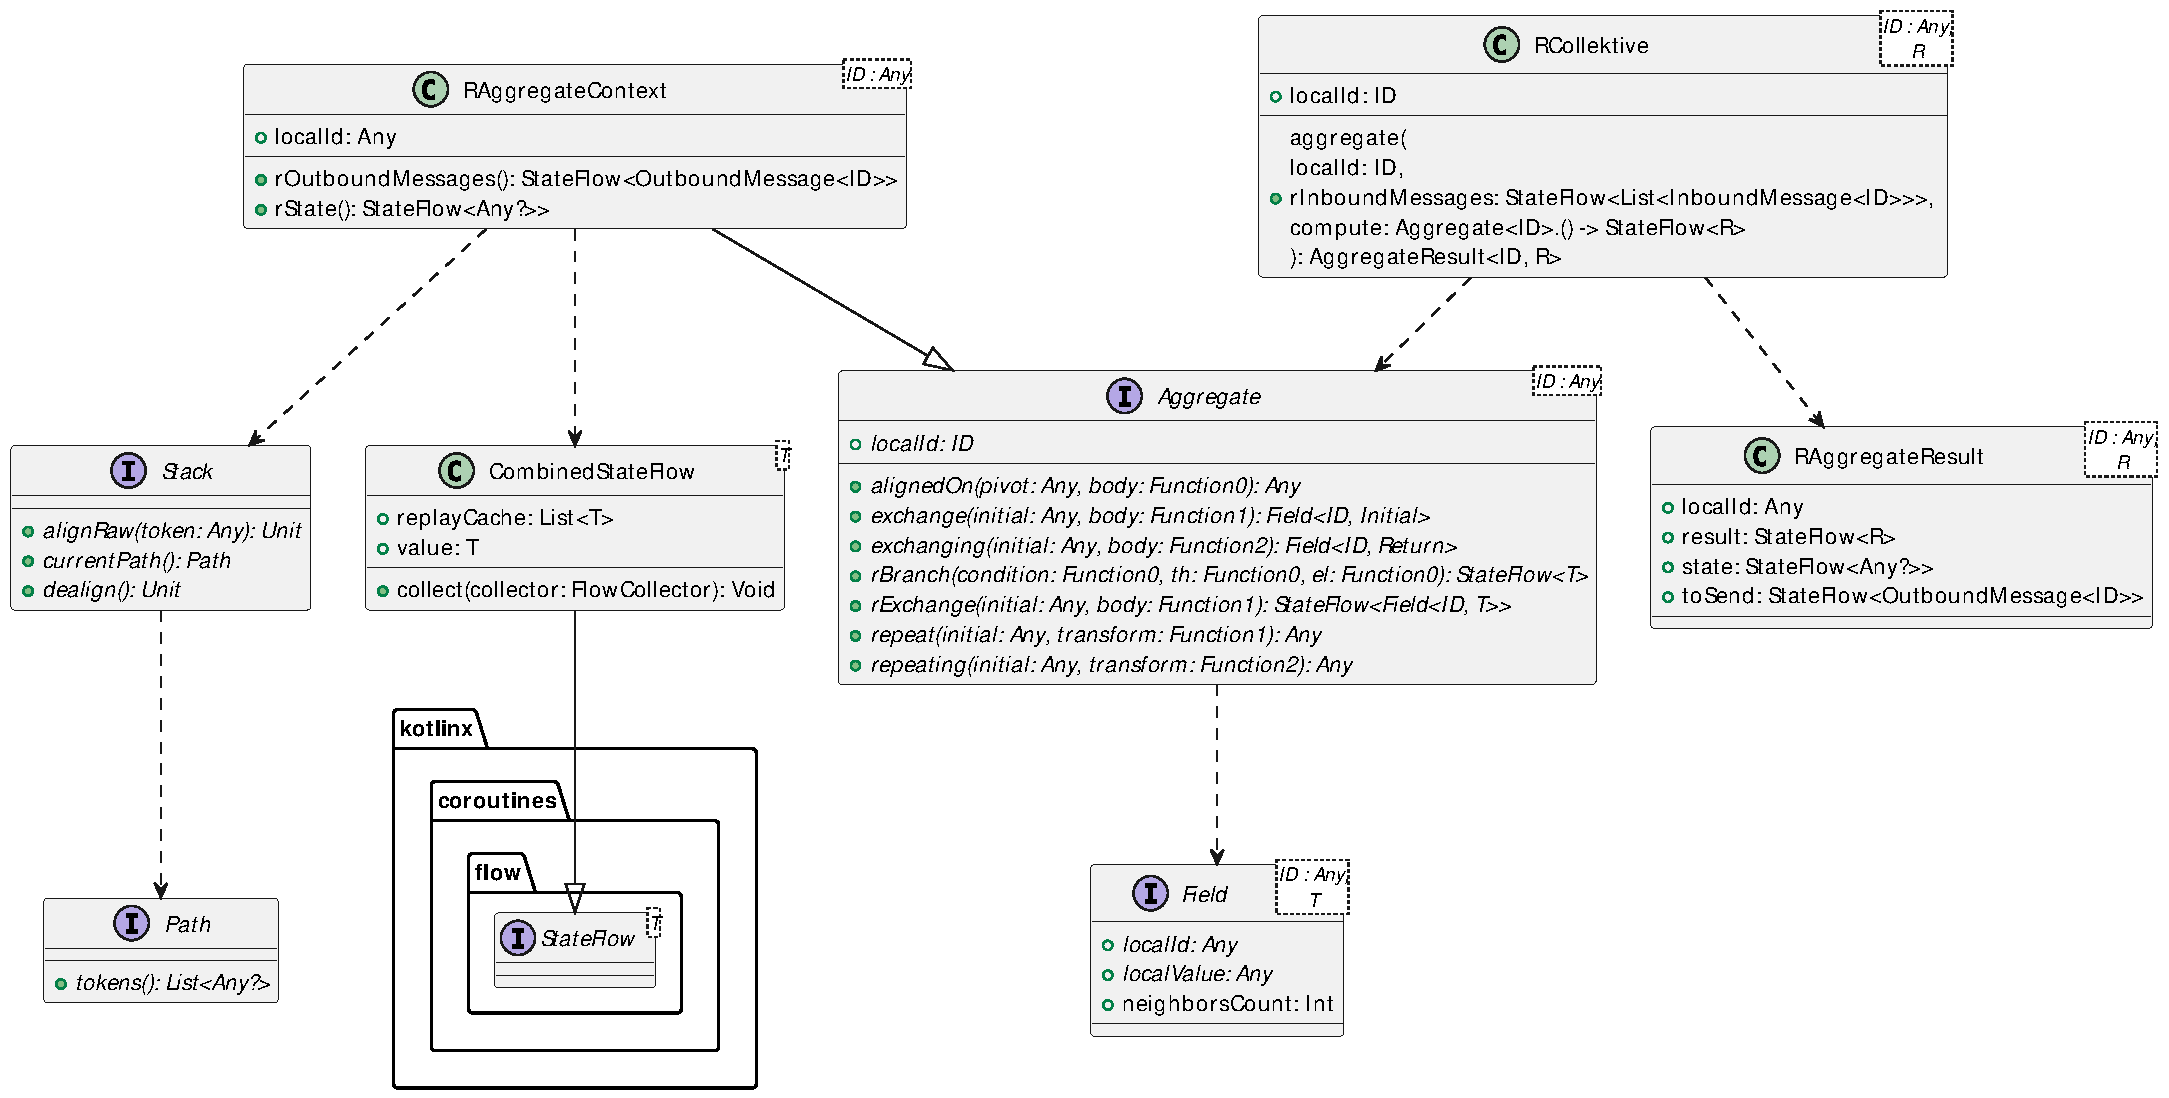
\includegraphics[width=\linewidth]{figures/collektive-prm-design.pdf}
    \caption{Detailed design of the purely reactive model proposed.}
    \label{fig:collektive-prm-design}
\end{figure}

\subsection{Model with Reactive Messages and Sensors}
The detailed design of the model with reactive messages and sensors is shown in \Cref{fig:collektive-rmsm-design}.

Similar to the purely reactive model, the \texttt{Collektive} class accommodates two new versions of the \texttt{Aggregate} method to facilitate reactive functionalities. These methods accept either a \texttt{StateFlow<Iterable<InboundMessage<ID>>>} or a \texttt{ReactiveNetwork<ID>} parameter, enabling dynamic adjustment of aggregate computations based on real-time changes in message reception.

In this model, the \texttt{Aggregate} method encompasses the logic necessary for reactive evaluation of the aggregate expression. Unlike the purely reactive model, where the \texttt{AggregateContext} class handles reactive evaluation, here the evaluation logic is embedded directly within the \texttt{Aggregate} method. Consequently, upon receiving a message from a neighbor, the entire aggregate expression undergoes reevaluation, resulting in a complete round of computation. While maintaining compatibility with the original Collektive \ac{dsl}, this approach sacrifices some performance due to the exhaustive reevaluation process.

\subsubsection{Behavioral Characteristics}

The model with reactive messages and sensors exhibits behavioral characteristics that align with its design principles:

\begin{itemize}
    \item \textbf{Compatibility}: Retains compatibility with the original Collektive \ac{dsl}, ensuring seamless integration with existing codebase and workflows.
    \item \textbf{Simplified Implementation}: Integrates reactive functionalities within the \texttt{Aggregate} method, streamlining the implementation process and reducing complexity.
    \item \textbf{Performance Trade-off}: Sacrifices some performance for compatibility, as the entire aggregate expression undergoes reevaluation upon receiving a message, potentially leading to redundant processing.
\end{itemize}

Despite the performance trade-off, this model provides a pragmatic approach to introducing reactivity into the Collektive framework, catering to scenarios where compatibility and ease of integration are paramount.

In summary, both models offer distinct approaches to incorporating reactive principles into the Collektive framework, each tailored to different use cases and design priorities.

\begin{figure}
    \centering
    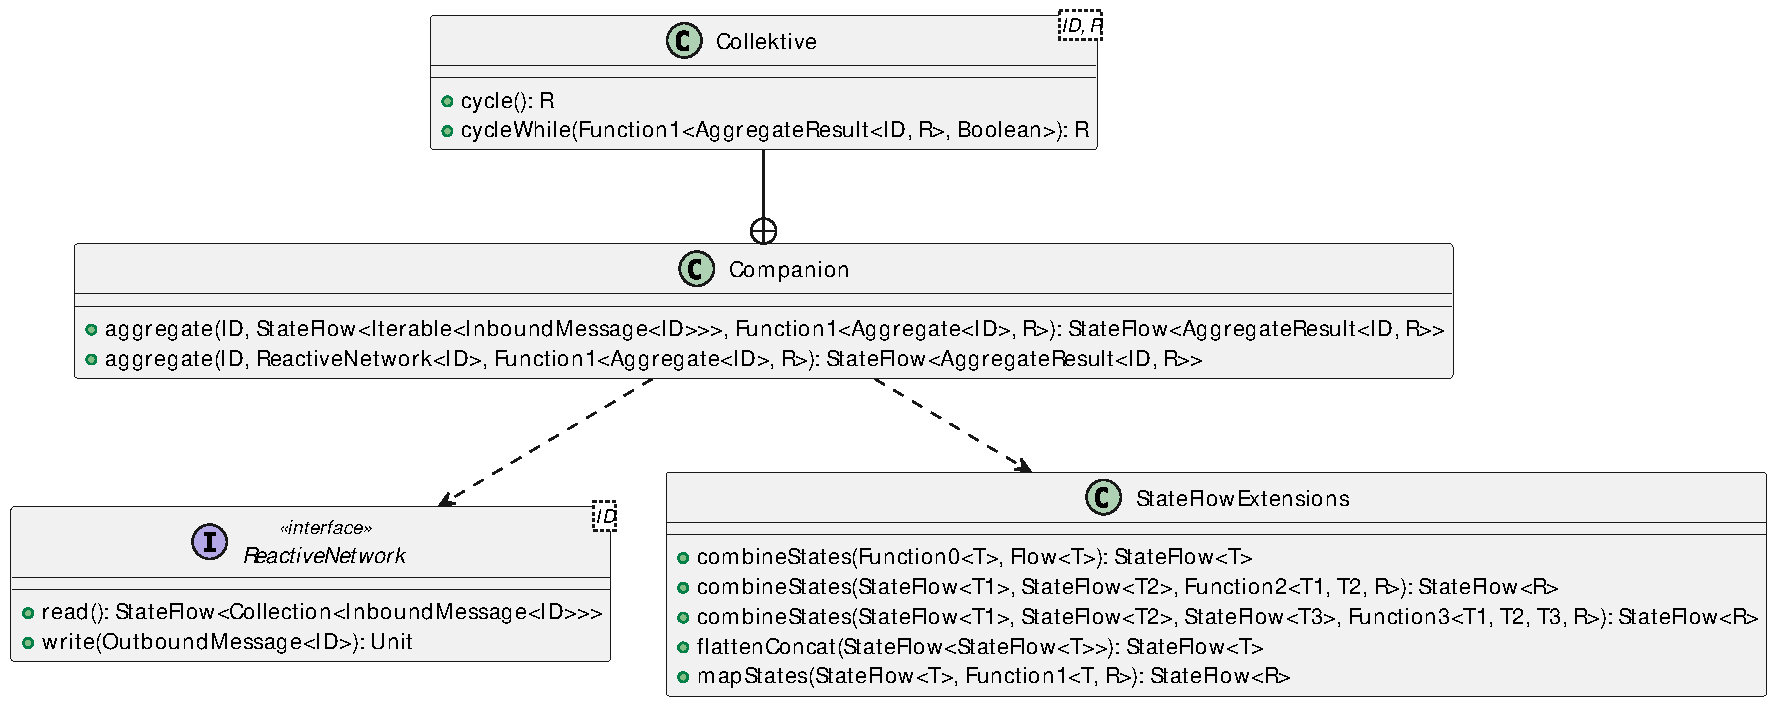
\includegraphics[width=\linewidth]{figures/collektive-rmsm-design.pdf}
    \caption{Detailed design of the model with reactive messages and sensors proposed.}
    \label{fig:collektive-rmsm-design}
\end{figure}
